\begin{comment}
	previous SOTA models used in obj detect VGG 16/30 layers
	intuitively deep learning improve with more layers
		resnets proved this was not necessarily the case
		poor performance when simply stacking layers
	denoted a degradation problem
		training accuracy was poor - not all systems easy to optimise
		accuracy becomes saturated
		not overfitting, as their is higher training error - harder to optimise
	 present a new idea
	 	construction with identity mapping
	 	added layers are identity mapping - all other layers copied from learned shallower model
	 	therefore, deeper model should have no higher training error than shallower counterpart
	 	current solvers unable to do this
 	introduce deep residual learning framework
 		instead of hoping few stacked layers directly fit a desired underlying mapping
 		let layers fit residual mapping - hypothesis that this is easier to optimise
 		similar to shortcut connections - show figure and equation
 		this performs the identity mapping, no extra parameters, minimal complexity (addition)
\end{comment}

\section{Residual Networks}
After the impressive advances of various challenges with ResNets in 2015 the use of these have become a standard for object detection systems, with many of the entries in \gls{mscoco} and \gls{ilsvrc} being based upon ResNets. The intuition of deep neural networks is that as the model becomes deeper richer representations of the original input are found. However, as shown in the work of ResNets \cite{deepres}, it is difficult to train deeper versions of commonly used \gls{cnn} architectures. Before the appearance of ResNets one of the standard architectures were VGG nets \cite{vgg16}, consisting of 16 to 30 layers. The intuition of deeper architectures lead to better networks was explored in \cite{deepres} by stacking additional layers and creating a 56 layer \gls{cnn}. It was found that stacked deeper networks have a degradation problem and the networks converge to a testing error higher than the corresponding shallower networks. A hypothesis could be made that this is due to a deeper network overfitting the dataset, however, it was determined that this was not the case as deeper models also exhibit higher training error. The solution to this degradation problem was to to construct deeper models using identity mapping and residuals, dubbed a deep residual learning framework. With this framework a given layer learns a residual mapping between the previous layer output and operations on the output. Using this reformulation the training error in the current layer should be no greater that the previous. This core concept of a residual block is visualised in \figref{resblock}. The input $x$ is passed into the block where a mapping is computed with two weight layers with convolutional operations with a \gls{relu} operation between them, representing an alteration with $F(x)$. After this the original input (identity) is added through a shortcut connection to the mapping by $F(x) + x$. This formulation forces the convolutional layers to compute weights to learn the residual mapping $F(x)$. 

\begin{figure}[H]
  \centering
    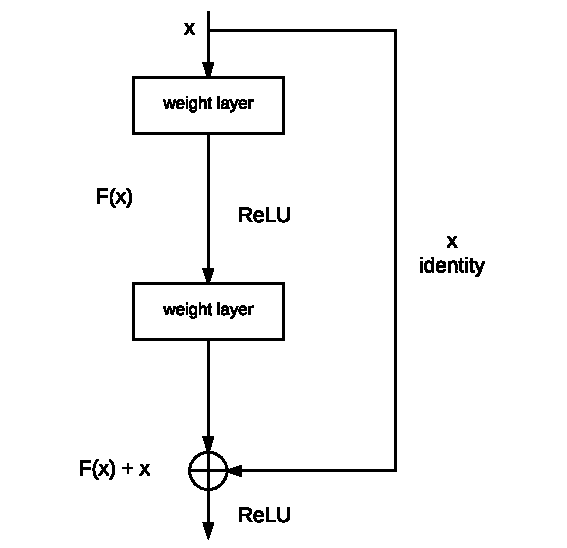
\includegraphics[width=0.5\textwidth]{Figs/Techanal/resblock.pdf}
    \caption{Core concept of residual blocks used in ResNets.}
    \label{fig:resblock}
\end{figure}

The formulation of $F(x) + x$ requires that the dimensions of $F$ and $x$ are equal. In situations where this is not the case a linear projection $W_sx$ is performed on $x$ such that the dimensions match. The final formulation of a residual block is:

\begin{equation}
	y = F(x, {W_i} + W_sx)
\end{equation}

where $W_i$ are the weights of the convolutional layers.

In the original work, experiments on a number of different architectures with residual blocks are conducted. Firstly, ImageNet classification is evaluated using naively stacked plain networks and ResNets. The plain networks are inspired by VGG nets \cite{vgg16} with two design criteria. Firstly, for a given output feature map size the number of filters must be equal. Secondly, if the feature maps size is halved the number of filters in the layer are doubled. The ResNets are variants of these plain networks but with residual connections in each block. In order to perform a fair comparison the linear projection performed in ResNets when dimensions are altered is done with zero-padding so that no extra parameters are added. Both sets evaluated are with 18 and 34 layers. An example of plain and ResNets can be seen in \figref{plainres}.

\begin{figure}[H]
  \centering
    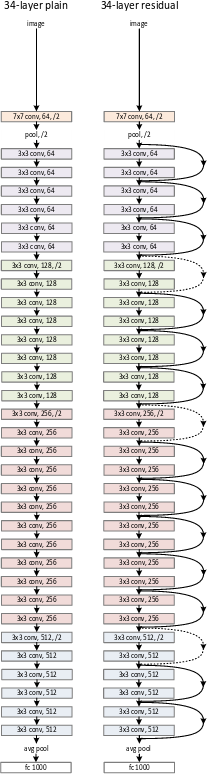
\includegraphics[width=0.1\textwidth]{Figs/Techanal/plainres.png}
    \caption{PLACEHOLDER. Overview of 34 layer plain and residual networks.}
    \label{fig:plainres}
\end{figure}

On top of the use of residual blocks, ResNets are also trained with scale augmentation and batch normalisation. During inference, multi-scale testing is conducted. Results on ImageNet validation top-1 error showed that the use of residual blocks aided in the optimisation of deeper architectures. \tableref{plainrestable} shows that the deeper plain networks exhibited troubles in optimisation with increased error with a deeper network. However, ResNets provided a decrease of 2.85\% between the two respective architectures.

\begin{table}[h]
\centering
\caption{Top-1 error(\%) on ImageNet validation set.}
\label{tab:plainrestable}
\begin{tabular}{|l|l|l|}
\hline
          & \textbf{plain} & \textbf{ResNet} \\ \hline
\textbf{18 layers} & 27.94 & 27.88  \\ \hline
\textbf{34 layers} & 28.54 & 25.03  \\ \hline
\end{tabular}
\end{table}

Haven shown that ResNets aid in optimisation of deep networks, the authors experimented with even deeper networks of 50, 101, and 152 layers. Due to concerns in the training time the residual blocks are altered in comparison to that shown in \figref{resblock}. The new block shown in \figref{newresblock}, $F$ consists of 3 convolutional layers of size $1 \times 1, 3 \times 3,$ and $1 \times 1$. The two sets of $1 \times 1$ layers are used to reduce complexity by reducing the input to the $3 \times 3$ layer and restoring the resulting output. 

\begin{figure}[H]
  \centering
    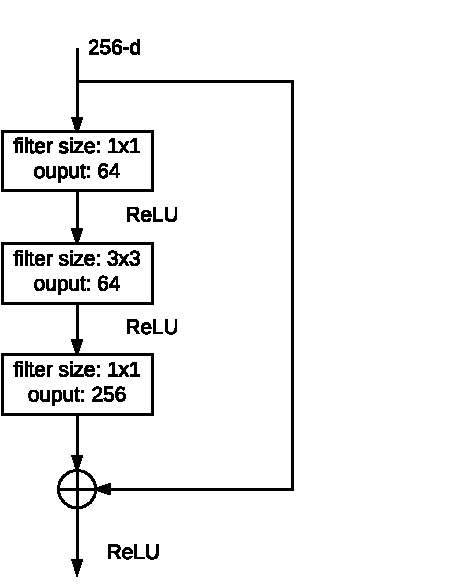
\includegraphics[width=0.5\textwidth]{Figs/Techanal/newresblock.pdf}
    \caption{Residual block used in deeper ResNet architectures.}
    \label{fig:newresblock}
\end{figure}


The deeper ResNets prove to give impressive results on the ImageNet validation sets as seen in \tableref{deepresimagenet}, with the very deep ResNet-152 providing the lowest error.

\begin{table}[]
\centering
\caption{Results of various deep ResNet architectures on ImageNet validation set.}
\label{tab:deepresimagenet}
\begin{tabular}{|l|l|l|}
\hline
\textbf{Method}     & \textbf{top-1 error (\%)} & \textbf{top-5 error (\%)} \\ \hline
\textbf{ResNet-34}  & 21.84            & 5.71             \\ \hline
\textbf{ResNet-50}  & 20.74            & 5.25             \\ \hline
\textbf{ResNet-101} & 19.87            & 4.60             \\ \hline
\textbf{ResNet-152} & 19.38            & 4.49             \\ \hline
\end{tabular}
\end{table}

